\chapter{Systementwurf}\label{chp:systementwurf}
%Auf der Basis des Pflichtenhefts werden aus softwaretechnischer Sicht die Anforderungen an das System spezifiziert. Hierzu gehört minimal eine Beschreibung auf höherem Niveau (Modulebene), eine auf mittlerem Niveau (Struktogramme, Pseudocode oder Spezifikation von Prozeduren (Funktionen) sowie die Beschreibung der für das System essentiellen Datenstrukturen (z.B. als Datenlexikon). Typische Beschreibungen sind die Modulhierarchie (oder Modulgraph), eine Spezifikation aller Module mit ihren Schnittstellen (inklusive Zweck, Ein-/Ausgabe), sowie eine Spezifikation aller in den Modulschnittstellen liegenden Prozeduren und Funktionen.
%Bestandteil des Entwurfs sollten nicht nur die jeweiligen Ergebnisse, sondern auch die Beschreibung des Entwicklungsweges (inklusive verworfener Lösungen) sein.

\section{Klasse Window}
\paragraph{}
Die Klasse \textit{Window} baut die Benutzeroberfläche auf und speichert die Eingabe des Benutzers in Variablen. Diese Werte werden dann an der Klasse \textit{Interpreter} weiter gegeben. In der Benutzeroberfläche werden die Eigenschaften für ein Testvorgang eingestellt.


\subsection{Design}
\begin{figure}[h]
  \begin{center}		%width=\linewidth
    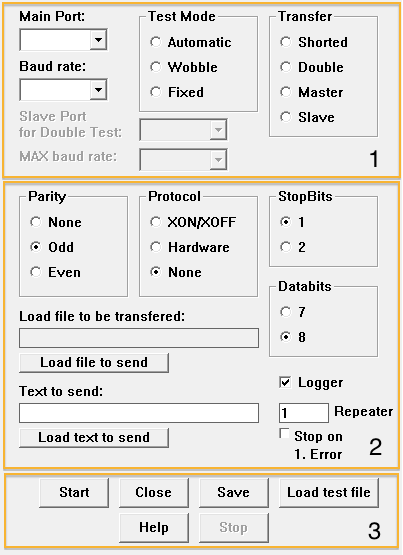
\includegraphics[scale=0.6]{gui.png}
  		  \caption{Design der Benutzeroberfläche}
  		  %\footnotesize{Quelle: www.pololu.com}
     \label{GUI_Bild}
  \end{center}
\end{figure}


Die Benutzeroberfläche ist in drei Abteilungen geteilt. Die verschidene Abteilungen sind in Abbildung \ref{GUI_Bild} zu erkennen. Genaueres zu alle Parametern wird in Kapitel ~\ref{chp:bedienungsanleitung} und  ~\ref{chp:fachlichesumfeld} erläutert. Die erste Reihe von Einstellungen hantieren die Testeinstellungen. Diese Einstellung sind:
\begin{itemize}
\item Main Port: welches COM Port soll getestet werden.
\item Baud rate: beschreibt mit welcher Baudrate der ausgewählte Port getestet werden soll.
\item Test Mode: definiert welcher Testvorgang der Benutzer haben will.
\item Transfer: legt fest, wie die Kommunikation dieses Ports stattfinden wird.
\end{itemize}


Die zwei ausgegraute Einstellungen ("`Slave Port for Double Test"' und "`MAX baud rate"') sind abhängig vor der Einstellungen in "`Test Mode"' und "`Transfer"'.\\

Die zweite Abteilung von Einstellungen sind die Übertragungsparameter und drei weitere Testeinstellungen. Diese Parameter sind:

\begin{itemize}
\item Parity: Paritätsüberprüfung.
\item Protocol: Übertragungsprotokoll.
\item Stopbits: Anzahl der Stopbits.
\item Databits: Anzahl der Datenbits.
\item Logger: definiert ob eine Log-Datei erstellt werden soll.
\item Repeater: Anzahl der Testwiederholungen.
\item Stop on 1. Error: bestimmt ob bei der ersten Fehlererkennung angehalten werden soll.
\item Load file to be transfered: Übertragungsdatei.
\item Text to send: Übertragungstext.\\
\end{itemize}

Die letzte Reihe von Elemente in der Benutzeroberfläche sind die Knöpfe. Diese führen die jeweilige Vorgange aus.

\begin{itemize}
\item Start: startet ein Test.
\item Close: schließt das Test Tool.
\item Save: speichert in eine Testdatei die Einstellungen.
\item Load test file: ladet eine Datei die im Test übertragen wird.
\item Help: zeigt ein Fenster mit Erklärungen zum Test Tool.
\item Stop: stoppt der laufende Test.\\
\end{itemize}

Bei drücken des Start-, Save- oder "`Load test file"'knopfes werden die Testeinstellungen an die Klasse \textit{Interpreter} weitergegeben und dort werden diese verarbeitet.


\subsection{Aufbau}
\paragraph{}
Die Klasse \textit{Window} erbt von der \textit{Template class} in die Headerdatei "`BaseWindow"'. Die Headerdatei beinhaltet die Definition des Templates. Im das Template wird die, für die Nachrichtenschleife nötige, statische Fensterprozedur deklariert. Hier wird nur nach der Nachricht \textit{WN\_NCCREATE} abgefragt, wie bereits im Kapitel \ref{C++GUILoesung} erwähnt. Wenn die Nachricht empfangen worden ist, werden die weitere Nachrichten an das Handle des Fensterobjekt weitergeleitet. In das Template wird außerdem auch eine Fensterklasse deklariert, registriert und danach erzeugt. Somit werden alle Nachrichten eines Fensterobjektes immer zuerst an die statische Fensterprozedur gesendet, diese leitet durch Zeiger und Handles die Nachricht an das korrekte Fenster. Um genauer die Funktionalität des Templates zu verstehen, bitte siehe Anhang \ref{TemplateClass}.

\subsection{Aufgaben}
\paragraph{}
Die Klasse hinter der Benutzeroberfläche besteht aus zwei Teilen. Das erste Teil bearbeitet die Eingabe des Benutzer und der Aufbau der Oberfläche, das zweite Teil die Weitererarbeitung der Daten.\\

Das erste Teil besteht aus die Methode \textit{HandleMessage}, diese Methode ist die Fensterprozedur. Als erstes werden die Elemente, mit der Ankunft der Nachricht \textit{WM\_CREATE}, des Fensters aufgebaut. Danach wird auf die Nachricht \textit{WM\_COMMAND} gewartet und jeweils reagiert. Wird zum Beispiel das Start Knopf gedrückt, bekommt die \textit{HandleMessage} Methode die \textit{WM\_COMMAND} Nachricht mit dem Parameter \textit{ID\_BT\_START}. Das ist die Identifikationsnummer im Programm für die Startschaltfläche.\\

\begin{lstlisting}	 
    case WM_CREATE:
        {
            //Create all GUI Elements
            
            //example: Start button
            _hwnd_Start = CreateWindowA("button", "Start",
				WS_CHILD | WS_VISIBLE,
				POS_X + 20, POS_Y2 + 290, 70, 30, m_hwnd, (HMENU)ID_BT_START,
				NULL, NULL);
        }
        break;
\end{lstlisting}

Wenn die Startschaltfläche gedrückt worden ist, fängt das zweite Teil der Klasse an. Das zweite Teil besteht aus die Weiterverarbeitung der Eingaben. Im Fall von der Startschaltfläche, wird als erstes einen neuen Thread aufgerufen. So kann die Benutzeroberfläche immer noch Nachrichten verarbeiten, während im Hintergrund, das Programm die Datenverarbeitung beginnt. Der gleiche Vorgang geschieht, wenn die \textit{Load test file} Schaltfläche gedrückt wird.\\

Im Fall von der Startschaltfläche, ruft das Thread die Methode \textit{sendTestSettings} auf, die die Eingaben weiter an ein Interpreter-Objekt gibt. Dies geschieht in dem ein Objekt der Klasse \textit{Interpreter} erzeugt wird und dessen Eigenschaften gesetzt werden.

\begin{lstlisting}	 
	case WM_COMMAND:
	{
		//React to GUI Elements actions
		//example: Start button
		case ID_BT_START:

			//hide the elements while testing
			viewAllElements(FALSE);

			//start a new thread
			_t1 = thread(&Window::sendTestSettings, this);

			//detach the thread so it can test and main thread waits
			//for it to finish or waits for the user to press stop
			_t1.detach();
	}
    break;
\end{lstlisting}




%****************************************************************************************
\newpage
%****************************************************************************************

\section{Klasse Interpreter}

Die Klasse \textit{Interpreter} trennt die Benutzeroberfläche von die Fachlogik des Programms. Die Benutzeroberfläche kann den Interpreter aufrufen und hat Zugriff auf die \textit{public} Methoden der Klasse. Der Interpreter kann nicht auf Elemente oder Methoden der Klasse \textit{Window} zugreifen. Durch diese Trennung kann der Benutzer nie "ùnkontrolliert"' auf die Fachlogik zugreifen, nur über die Möglichkeiten die der Programmierer anbietet.\\

\subsection{Aufgaben}
\paragraph{}
Eine Aufgabe des Interpreters ist die Überprüfung der Eingaben des Benutzers bevor die Tests beginnen. Durch "`setter"' Methoden werden die Eingabeparameter der GUI in lokalen Variablen gespeichert.\\


\begin{lstlisting}	 
void Interpreter::setTransfer(int iTransfer)
{
	this->_iTransfer = iTransfer;
}
\end{lstlisting}

Danach werden die lokalen Variablen auf Fehleingaben geprüft. Sind Fehler erkannt worden, werden diese dem Benutzer bekannt gemacht und alle Parameter in der Klasse werden auf ein Standardwert zurückgesetzt. Sind keine Fehleingaben erkannt, werden die Werte der Variablen in einer Datenstruktur gespeichert. Mehr zu dieser Struktur erfahren sie im Kapitel ~\ref{TestStruct}. Folgende Codezeilen stellen dar, wie ein Fehlerüberprüfvorgang aussieht. Hier wird nach dem Übertragungsmodus abgefragt.

\begin{lstlisting}	 
if (_iTransfer == DEFAULT_VALUE)
{
	MessageBoxA(NULL,"Bitte wählen Sie ein Transfermodus aus",
							WINDOW_TITLE, MB_OK | MB_ICONERROR);
	setDefaultValues();
}
else
{
	//speichern des Transfermodus
	_testManager->testStruct.iTransfer = _iTransfer;
}
\end{lstlisting}

Die Werte in den Variablen müssen überprüft werden, um Fehler zu vermeiden. Da die Werte nicht nur aus Einstellungen in der Benutzeroberfläche stammen, sondern auch aus eine Testkonfigurationsdatei, können falsche Eingabe vorhanden sein.\\

Außer die Überprüfung der Eingabeparameter und setzen der lokalen Variablen, gibt diese Klasse die Testeinstellungen an die anderen Klassen weiter. Hier trennt sich das Programm in zwei Pfade. Das erste Pfad gibt die Datenstruktur an die Klasse \textit{TestManager} weiter. Der zweite Pfad speichert oder liest eine Testkonfigurationsdatei. Im Fall, dass eine Testkonfigurationsdatei gelesen werden soll, wird als erstes die Klasse \textit{IniFileHandler} aufgerufen und danach die Klasse \textit{TestManager}, damit ein Test mit den gelesenen Einstellungen gestartet wird. Sollen die Eingabeparameter der Benutzeroberfläche in einer Testkonfigurationsdatei gespeichert werden, werden die überprüfte Eingabeparameter in einer vom Benutzer angegebene Datei gespeichert. Dafür wird auch die Klasse \textit{IniFileHandler} aufgerufen.\\

Da die Klasse \textit{Interpreter} die Schnittstelle für die Kommunikation zwischen Fachlogik und Benutzer ist, wird auch durch diese Klasse die Meldung gegeben, ein Test anzuhalten. Durch das Klicken der Schaltfläche "`Stop"' in der Benutzeroberfläche wird eine boolesche Variable weiter an die Testlogik gegeben. Diese Variable wird vor jedem Testschleife abgefragt, ist sie gesetzt, dann wird das Testen angehalten.\\

Die Klasse hat ein Objekt der Klasse \textit{Com}, um in der Benutzeroberfläche die im System zur Verfügung stehende COM Ports aufzulisten. Durch die Trennung der GUI mit der Fachlogik, darf die \textit{Window} Klasse kein Objekt der Klasse \textit{Com} haben.\\



%****************************************************************************************
\newpage
%****************************************************************************************

\section{Struktur TestStruct}\label{TestStruct}
\paragraph{}
Ein \textit{struct} oder Struktur dient dazu, mehrere logische zusammenhängende Variablen verschiedener Datentypen zusammenzufassen. In \textit{C} beinhalten Strukturen nur Variablen, in \textit{C++} wurden die Strukturen erweitert und dürfen auch Funktionen beinhalten. Dadurch ist der Unterschied zu einer Klasse nur die Zugriffsrechte auf die Eigenschaften. In einer Struktur sind die Zugriffsrechte auf Elemente mit  \textit{public} definiert, in einer Klasse mit \textit{private}\footnote{\cite{VisualC++}}. Da ich nur Variablen benötigte, und keine Methoden, habe ich mich für eine Struktur entschieden.


\subsection{Aufbau}
\paragraph{}
Die Datenstruktur fasst alle Eigenschaften für einem Test zusammen. Die \textit{TestStruct} beinhaltelt folgende Variablen und wird so definiert:\\

\begin{lstlisting}	 
struct TestStruct
{
	string sMasterPort;
	string sSlavePort;
	string sTextToTransfer;
	string sFilePath;
	int iTransfer;
	int iBaud;
	int iBaudrateMax;
	int iTestMode;
	int iParity;
	int iProtocol;
	int iStopbits;
	int iDatabits;
	int iTransTextMode;
	int iRepeater;
	bool bLoggerState;
	bool bStopOnError;
	vector<string> svBaudrates;
}
\end{lstlisting}

Jeder dieser Variablen stellt ein Wert dar, für eine Einstellung in der Benutzeroberfläche. Für eine genauere Erläuterung der Variablen und dessen Werte, bitte siehe Kapitel \ref{chp:bedienungsanleitung} und ~\ref{IniFileHandler}.

%****************************************************************************************
\newpage
%****************************************************************************************


\section{Klasse Com}
\paragraph{}
Die Klasse \textit{Com} umfasst alles um die Verwaltung eines COM Ports. Um aus einem COM Port lesen und schreiben zu können, müssen zuerst die Eigenschaften des jeweiligen Ports gesetzt werden. Alle Ports in einem System werden beim Systemstart mit einer Standardkonfiguration konfiguriert. Will der Benutzer Peripherieelemente an einem COM Port anschließen, die nicht die gleiche Konfiguration besitzt wie die im System vordefiniert, muss die Konfiguration des Ports angepasst werden. Dafür muss ein COM Port zuerst geöffnet werden, danach kann die Konfiguration geändert werden. Wenn diese beide Schritte erfolgreich abgelaufen sind, können aus dem COM Port Informationen gesendet und empfangen werden. Als letzter Schritt ist sehr wichtig der öffene COM Port wieder zu schließen. Somit steht der COM Port wieder andere Applikationen und das System zur Verfügung.\\

\subsection{Aufgaben}
\paragraph{}
Um einem COM Port zu öffnen, wird die gleiche Systemfunktion aufgerufen, wie um eine Datei zu erzeugen. Die Funktion \textit{CreateFile} gibt ein Handle auf das gewünschte COM Port. Durch dieses Handle wird der jeweilige Port für andere Operationen identifiziert.

\begin{lstlisting}	 
hCom = CreateFile(portNumber.c_str(),  
            GENERIC_READ | GENERIC_WRITE,
            0, 
            NULL,
            OPEN_EXISTING, 
            FILE_FLAG_OVERLAPPED,
            NULL); 

\end{lstlisting}

Das erste Parameter der Funktion ist der Name des gewünschtes Ports. Besitzt der COM Port einen Wert von eins bis neun wird ein Wert wie "`COM5"' gesetzt. Ist der Wert des Ports größer neun und maximal 256, muss der erste Parameter folgendermaßen gesetzt werden: "`\textbackslash\textbackslash.\textbackslash COM255"'. Der zweite Parameter beschreibt die Zugriffsrechte auf der COM Port. Da wir Informationen senden und empfangen möchten, braucht das Programm Lese- und Schreibrechte. Sehr wichtig ist der fünfte Parameter. Dieser beschreibt das nur existierende COM Ports geöffnet werden sollen. Da die Funktion auch Dateien erzeugen kann, sind diese nicht vorhanden, werden sie kreiert. Im Fall von COM Ports,  keine COM Ports sollen erzeugt werden, sondern die als Hardware im System vorhanden öffnen. \textit{FILE\_FLAG\_OVERLAPPED} setzt die Eingenschaft, dass der COM Port im asynchron Modus geöffnet werden soll.\\

Damit den Benutzer, in der Benutzeroberfläche, nicht vorhandene COM Ports angeboten werden, wird bei der Aufbau der GUI alle zur Verfügung stehende COM Ports aufgelistet. Dafür wird in einer Schleife versucht alle COM Ports zwischen Null bis 256 zu öffnen, alle die Ports die einen gültigen Handle zurück geben werden aufgelistet.\\


Wenn ein COM Port nicht erfolgreich geöffnet werden konnte, gibt die \textit{CreateFile} Funktion ein nicht valides Handle zurück. Wird ein Port erfolgreich geöffnet, können die Eigenschaften des Ports bearbeitet werden. Wie in Unterkapitel \ref{COMWINAPI} erklärt, werden die Eigenschaften des Ports durch verschiedene Strukturen gesetzt.\\

Für jeden Test kann der Benutzer die Baudrate einstellen. In der Benutzeroberfläche wird in Form einer Liste, in einer "`Combo Box"', die unterstützten Baudrate aufgelistet. Um die Baudraten zu ermitteln muss zuerst die Struktur \textit{COMMPROP} geladen werden. In der Variable \textit{dwSettableBaud} sind als Bitmaske die unterstützten Baudraten gespeichert. Das Algorithmus dafür sieht so aus:

\begin{lstlisting}
	//Lade die COMMPROP Stuktur des geöffneten Ports	 
	GetCommProperties(hCom, &commProp);
 
 	//Bitmaske mit den unterstützten Baudraten
	bitset<32> bitMask ((int)commProp.dwSettableBaud);
	
	//ignoriere die letzte 4 bits
	for( int i = 0; i < 28; i++)
	{
		//falls das Bit gesetzt ist
		if (bitMask.test(i) == true)
		{
			//dann wird die Baudrate unterstützt
			vBaud.push_back(saDefaultBaudrates[i]);
		}
	}
\end{lstlisting}

In der Schleife wird geprüft ob der jeweilige Bit an der Stelle "`i"' eine Eins oder Null ist. Falls es eine Eins ist, dann wird die Baudrate im Array an der Stelle "`i"' in eine Vektor gespeichert. In diesem Vektor werden alle Baudraten gespeichert, die vom angegebene Port unterstützt werden. Der Vektor gehört zur \textit{Com} Klasse und wird durch das ganze Programm benutzt.\\

Die Timeoutwerte für Lese- und Schreibzugriffe werden auch in dieser Klasse berechnet und gesetzt. Dafür muss eine  Struktur \textit{COMMTIMEOUTS} deklariert werden. Die Struktur wird nach .....Wünsch und Zweck..... des Programms bearbeitet. Für das Test Tool werden in der Struktur die Zeit für die Übertragung eines Zeichens geschrieben. Für die Berechnung für dieses Wert und die Erklärung siehe bitte Unterkapitel ~\ref{COMWINAPI}.

\begin{lstlisting}
	//Port Timeout Struktur
	COMMTIMEOUTS timeouts;
	
	timeouts.ReadIntervalTimeout				 = 20;
	timeouts.ReadTotalTimeoutMultiplier	 = iTimeOut;
	timeouts.ReadTotalTimeoutConstant		 = 100;
	timeouts.WriteTotalTimeoutMultiplier = iTimeOut;
	timeouts.WriteTotalTimeoutConstant	 = 100;
	
	SetCommTimeouts(hCom, &timeouts);
\end{lstlisting}

Durch die Funktion \textit{SetCommTimeouts} mit Angaben des geöffneten Ports und eine Referenz auf einer Variable der Struktur \textit{COMMTIMEOUTS} werden die Timeouts gesetzt. Davor müssen die Elemente von der Struktur initialisiert werden. Die Werte \textit{ReadTotalTimeoutMultiplier} und \textit{WriteTotalTimeoutMultiplier} werden mit der berechnete Zeit pro Zeichen gesetzt. Für die andere drei Variablen worden die empfohlene Werte aus der MSDN Online Bibliothek\cite{SerialCommunications} übernommen. \\

Objekte der Klasse \textit{Com} können durch der Aufruf von zwei verschiedene Konstruktoren erzeugt werden. Der erste Konstruktor ist der Standardkonstruktor, dieser wird für die Auflistung von die zur Verfügung stehende Ports und dessen Baudraten verwendet. Der zweite Konstruktor bekommt als Parameter ein String mit dem Namen des Ports. Dieser Port wird geöffnet und die Eigenschaften werden in lokale Variablen geladen und  für zukünftige Operationen in den Tests gespeichert.
 
%****************************************************************************************
\newpage
%****************************************************************************************


\section{Klasse PortCommunications}\label{PortCommClass}
\paragraph{}
In der Klasse \textit{PortCommunications} werden die Lese- und Schreiboperation ausgeführt. Die Klasse besteht aus zwei Konstruktoren, drei Methoden und ein Destruktor. Obwohl die Klasse nur aus drei Methoden besteht, diese ist die Klasse die tatsächliche Systemaufrufe für Senden und Empfangen von Daten befasst.\\

Die erste Methode in der Klasse speichert ein Handle von ein offenen COM Port in einer lokalen Variable. Durch dieses Handle weist die Klasse aus welchem Port die Lese- oder Schreibmethoden ihre Zugriffe ausüben sollen. Dieses Handle kann auch durch den Aufruf eines personalisiertes Konstruktor gesetzt werden, dass als Parameter an den Konstruktor übergeben wird.\\

Das Schreiben zu einem COM Port ist sehr ähnlich wie das Lesen. Beide Operationen werden in einer Schleife wiederholt bis alles Bytes aus dem Puffer gelesen worden sind. Der ganze Programmcode zu diesen Methoden kann in Anhang ~\ref{ReadDataCode} und ~\ref{WriteDataCode} gelesen werden. Im folgenden werden nur Ausblicke der beiden Vorgänge erklärt.\\

\subsection{Schreiben}
\paragraph{}
Die Methode \textit{writeData} erhält als Parametern der zu übertragene Text und die Länge des Textes. Die Länge des Textes ist für den Schreibvorgang nötig, damit die Schreibmethode ermitteln kann, wenn alle Bytes geschrieben worden sind. Bevor der Schreibvorgang beginnt, muss eine \textit{OVERLAPPED} Struktur deklariert werden, zuständig für das asynchrone Schreiben. In der Struktur wird die Variable \textit{hEvent} initialisiert, in dem ein neues Event deklariert wird.\\

Der Schreibvorgang wird in einer Schleife, die im Fehlerfall maximal fünf mal wiederholt wird, ausgeführt. In der Schleife wird die Methode \textit{WriteFile} folgendermaßen aufgerufen:
\begin{lstlisting}
	WriteFile(hCom, lpBuf, dwSize, &dwWritten, &osWrite);
\end{lstlisting}

Als Parameter benötigt die Methode das Handle aus dem Port wo gelesen werden soll. Somit kann die Methode in den verschiedene Testmodi der Sender und Empfänger unterscheiden. Als zweiter Parameter wird der zu schreibende Text und als dritter Parameter die Länge des Textes übergeben. Der vierte und fünfte Parameter sind die Adresse der jeweiligen Variablen. In der Variable \textit{dwWritten} werden die Anzahl der geschriebene Bytes geschrieben und die\textit{osWrite} Variable ist die am Anfang des Schreibvorgang erstellte \textit{OVERLAPPED} Struktur. War der Schreibversuch Fehlerhaft, wird es dem Benutzer ermittelt, sonst wird die Methode \textit{WaitForSingleObject} aufgerufen.

\begin{lstlisting}
	WaitForSingleObject(osWrite.hEvent, INFINITE);
\end{lstlisting}

Die Methode \textit{WaitForSingleObject} bekommt als Parametern das am Anfang kreierte Event in der \textit{OVERLAPPED} Struktur und eine Ablaufzeit. Die Methode wartet so lange bis das Event signalisiert wird. Im diesem Fall ist das Timeout auf \textit{INFINITE} gesetzt, damit das Schreiben vollständig beendet wird. Dieser Wert habe ich als Empfehlung aus der MSDN Online Bibliothek\cite{SerialCommunications} entnommen. Wenn das Event signalisiert wird, wird die Methode \textit{GetOverlappedResult} auf dieser Weise aufgerufen:

\begin{lstlisting}
	GetOverlappedResult(hCom, &osWrite, &dwWritten, FALSE);
\end{lstlisting}

Wieder bekommt die Methode das Handle auf das COM Port, die Adresse der \textit{OVERLAPPED} Struktur und die Adresse der Variable \textit{dwWritten}. Das letzte Parameter spezifiziert ob auf das Event gewartet werden soll. Da aber in \textit{WaitForSingleObject} schon gewartet wird, bis das Event signalisiert wird, muss bei dem Aufruf von \textit{GetOverlappedResult} nicht nochmal gewartet werden, deswegen wird der letzte Parameter mit \textit{FALSE} belegt.\\

Wenn die Methode \textit{GetOverlappedResult} \textit{FALSE} zurückliefert, wird der Benutzer den letzten Fehler benachrichtigt. Ist der Rückgabewert der Methode \textit{TRUE}, bedeutet es, dass der Schreibzugriff beendet worden ist. Um zu Erfahren ob der Zugriff erfolgreich war, werden die Variablen mit den zu schreibende Bytes und die geschriebene Bytes verglichen. Wenn diese Werte sich von einander unterscheiden, dann ist die Zeit für den Schreibzugriff abgelaufen (time out). Sind beide Werte gleich, dann war die der Vorgang erfolgreich und die Schreibmethode wird beendet.


\subsection{Lesen}
\paragraph{}
Die Lesemethode erhält die gleiche Parameter wie die Schreibmethode. Sie braucht auch eine \textit{OVERLAPPED} Struktur um das Event abfragen zu können. Das Grundgerüst für die Lesemethode ist der gleiche wie die von der Schreibmethode. Beide Vorgänge werden in einer Schleife wiederholt, bis der Vorgang beendet wird oder ein Fehler gemeldet wird. Der Unterschied ist das beim Lesen die Schleife nicht fünf mal wiederholt wird, sonder die Schleife ist unendlich. Obwohl das programmiertechnisch nicht empfehlenswert ist, muss die Leseoperation so oft wiederholt werden, bis alle Bytes angekommen sind. Der Empfänger muss diese Daten durch ein Pollingverfahren aus dem Puffer lesen. Die Methode zum Lesen lautet:

\begin{lstlisting}
	ReadFile(hCom, ourBuf, dwSize, NULL, &osReader)
\end{lstlisting}

Die \textit{ReadFile} Methode bekommt die gleiche Parameter wie die Schreibmethode. Der Unterschied ist, dass durch die asynchrone Kommunikation die Lesemethode nicht die Anzahl der gelesene Bytes speichert, weil diese verfälscht sein können. Wird der Lesezugriff Fehlerhaft ausgeführt, wird der Benutzer benachrichtigt, ansonsten werden die Methoden \textit{WaitForSingleObject} und \textit{GetOverlappedResult} aufgerufen. Die \textit{WaitForSingleObject} Methode bekommt als Ablaufzeit ein vordefiniertes Wert von 500 Millisekunden \footnote{\cite{SerialCommunications}}. Die Methode \textit{GetOverlappedResult} bekommt die gleiche Parameter wie im Schreibzugriff.\\

Um zu ermitteln ob der Lesevorgang erfolgreich abgeschlossen worden ist, müssen die Anzahl der gelesene Bytes mit der Anzahl der zu lesende Bytes verglichen werden. Da die Lesemethode mehrmals aufgerufen wird, werden bei jedem Vorgang nicht die ganze Anzahl an Bytes gelesen. Die gelesene Bytes müssen in einem Puffer gespeichert werden, ohne die schon gelesene Bytes zu überschreiben. Um dieses Problem zu lösen, wird ein Zeiger deklariert, der auf dem Anfang des Puffers im ersten Lesezugriff zeigt. Mit Hilfe von Zeigerarithmetik, wird der Zeiger immer um die gelesene Anzahl von Bytes addiert. Um zu ermitteln wann alle Bytes gelesen worden sind, wird einer Variable die Anzahl an gelesenen Bytes subtrahiert. Wenn diese Variable gleich Null ist, dann worden alle Bytes gelesen und der Lesevorgang wird erfolgreich abgebrochen. Um ein Fehler im Lesevorgang zu erkennen, darf eine Leseoperation maximal fünf mal in ein time-out geraten, dann wird der Vorgang abgebrochen und der Benutzer wird benachrichtigt.



%****************************************************************************************
\newpage
%****************************************************************************************


\section{Klasse TestManager}
\paragraph{}
Die Klasse \textit{TestManager} bereitet die Testeinstellungen und die Testlogistik vor. In der Klasse werden die letzten Parameter überprüft, besonders für den Wobbelntest, und verschiedene Variablen auf seine Standardeinstellung gesetzt, damit der Testvorgang fehlerfrei beginnen kann.


\subsection{Aufbau}
\paragraph{}

Die Klasse besteht aus vier Methoden, wo drei die Klasse \textit{FixedTest} (Kapitel~\ref{FixedTextClass}) aufrufen und die Test beginnen. Die andere Methode bereitet die Eigenschaften der Klasse \textit{TestManager} vor um die drei anderen Methoden aufrufen. Die Methode \textit{startManager} erzeugt ein Objekt der Klasse \textit{Logger} (Kapitel~\ref{LoggerClass}) wenn die Log-Option gesetzt ist. Danach werden die lokalen Variablen auf seine Standardwerte gesetzt und je nach Testeinstellung wird die richtige Testmethode aufgerufen.\\

Es gibt drei Testmodi (Fixed, Wobble und Automatic), und jedes Testmodi hat verschiedene Testeinstellungen. Im Fall von \textit{Fixed}, werden alle mögliche Test und Port Einstellungen berücksichtigt. Im \textit{Wobble} Test wird zwischen eine Unter- und Obergrenze der Baudrate und / oder der Parität gewobbelt. Der \textit{Automatic} Test ist ein vordefiniertes Testfall. Hier muss der Benutzer nur der zu testende COM Port auswählen und welche Transfermöglichkeit er sich wünscht.\\

Im Fall von einem \textit{Fixed} Test, wird in der Methode \textit{startManager} die Methode \textit{startFixedTest} aufgerufen. In der Methode \textit{startFixedTest} wird als erstes ein Objekt der Klasse \textit{FixedTest} erzeugt mit der aktuellen Teststruktur als Übergabeparameter. Ein Schleifenzähler wird initialisiert, dieser repräsentiert der \textit{Repeater} aus der GUI oder Konfigurationsdatei. Wenn die Log-Option gesetzt ist, wird die Testeinstellungen in einer Testkonfigurationsdatei gespeichert. Als nächstes in einer "`\textit{do while}"' Schleife werden die Methoden des Objektes \textit{FixedTest} aufgerufen, abhängig von die  Transfereinstellung (Shorted, Double, Master, Slave). Ist der Transfermodus \textit{Master} gesetzt, werden drei Sekunden gewartet, damit der Benutzer Zeit hat, das \textit{Slave} Modul in einem anderen System zu starten. Die Schleife wird wiederholt so lange der Schleifenzähler nicht seine Grenze erreicht oder der Benutzer den Test abbricht (durch drücken der Stopp-Schaltfläche in der Benutzeroberfläche oder der "`ESC"' Taste in der Kommandozeile). Ist die Option "`stop on first error"' gesetzt und ein Fehler in der Kommunikation wird erkannt, so wird auch die Schleife unterbrochen und der Errorcode zurückgegeben.\\

Hat der Benutzer ein \textit{Wobble} Test eingestellt, ist der Ablauf der Testvorbereitungen und Abbruchkriterien gleich wie in einem \textit{FixedTest}. Der einzige Unterschied zu einem \textit{Fixed} Test ist, dass zu einer Verschachtlung von Schleifen kommt. In diesem Test wird zwischen eine minimale und maximale Baudrate gewobbelt. Dafür werden alle Standard einstellbare Baudraten zwischen den Grenzen betrachten. Möchte der Benutzer auch durch die drei verschiedene Paritätseinstellungen (gerade, ungerade oder keine Parität) wobbeln, gibt es eine zweite Schleife, wo diese Eigenschaft wechseln eingestellt wird. So wird im ....breiten - längsten..... Testfall für eine  Baudrate die drei verschiedene Paritätseinstellungen eingestellt und für jede Paritätseinstellung der Test so oft wiederholt, wie im \textit{Repeater} angegeben.\\

Der \textit{Automatic} Test besitzt eine vordefinierte Testeinstellung. Für den angegebene COM Port wird eine feste Testkonfiguration gesetzt und diese so lange wiederholt, bis der Benutzer mit einem Abbruchkriterium den Test beendet. Für weitere Informationen über die Testeinstellungen und Testeigenschaften bitte siehe Kapitel ~\ref{chp:bedienungsanleitung}.

%****************************************************************************************
\newpage
%****************************************************************************************


\section{Klasse FixedTest}\label{FixedTextClass}
\paragraph{}
Die Klasse \textit{FixedTest} ist die Klasse die Kommunikation zwischen ein oder zwei COM Ports organisiert. Alle Testeinstellungen und organisatorisches wurde schon eingestellt. Die Klasse besitzt Objekte der Klassen \textit{PortCommunications} und \textit{Com}, um COM Ports zu verwalten und zwischen Ports zu kommunizieren.\\

\subsection{Ablauf eines Tests}
\paragraph{}
Für ein Test muss als erstes die ausgewählte Schnittstelle mit den ausgewählten Einstellungen eingestellt werden, unabhängig davon was für ein Testfall betrachtet wird. Die \textit{Master} und \textit{Slave} Tests sind komplexer als ein \textit{Shorted} oder \textit{Double} Test. Als erstes muss der ausgewählte Port geöffnet werden und die Port Eigenschaften geladen werden. Mit dem Aufruf der Methode \textit{setPortSettings} werden die angegebene Schnittstelleneinstellungen für den Test eingestellt. Im Fall von einem \textit{Shorted} Test muss nur eine Schnittstelle initialisiert werden. Ist es ein \textit{Double} Test müssen die ausgewählte Ports mit den gleichen Parametern initialisiert werden.\\

Ist dieser Schritt erfolgreich abgeschlossen worden, dann kann der Informationsaustausch beginnen. In einem \textit{Shorted} Test sendet und empfängt die gleiche Schnittstelle die Information. Diese wird verglichen um Fehler bei der Übertragung zu ermitteln. Ist es ein \textit{Double} Test, gibt es getrennte Sender und Empfänger. Da aber beide Schnittstellen sich im gleichen System befinden, kann die gesendete und empfangene Information auch verglichen werden. Das Ergebnis des Vergleichs wird in einem Vektor geschrieben, der am Ende der Übertragung als Ergebnis ausgegeben wird. Wurde die Option "`stop on first error"' gesetzt und ein Unterschied wurde im Vergleich erkannt, dann wird der Testvorgang abgebrochen. Wenn das Ende der Übertragungsinformation (eine Zeile, eine Datei oder der vordefinierte Text) erreicht wird, werden die geöffnete Schnittstellen geschlossen und das Testergebnis dem Benutzer gemeldet. Dieser Vorgang wird so oft wiederholt, wir es im \textit{Repeater} angegeben worden ist.\\

Zuständig für die Kommunikation einer Schnittstelle ist die Klasse \textit{PortCommunications}(siehe Kapitel \ref{PortCommClass}, für den Zugriff auf die Lese- und Schreibmethoden gibt es jeweils einer "`Wrapper"' Methode, die unter Master und Slave Schnittstellen unterscheidet. So bleibt die Testlogik getrennt von der Kommunikationslogik.

\subsection{Master und Slave}
\paragraph{}
Der Grundgerüst für ein \textit{Master} und \textit{Slave} Testvorgang ähnelt sich zu einem \textit{Shorted} Test. Der wesentliche Unterschied liegt an das Problem, das beide Schnittstellen sich nicht kennen und müssen synchronisiert werden. Als erster werden beide Schnittstellen für ein Test vorbereitet, das hießt, die COM Ports werden geöffnet, aber anstatt die Porteigenschaften auf die Testeinstellungen zu setzen, werden hier die Default-Einstellungen benutzt. Der Slave kennt die Testkonfiguration nicht, er kennt nur wie oft ein Test wiederholt wird und welcher Transfermodus er hat.\\

Die Synchronisation der beiden COM Ports geschieht indem der Master ein Fluchtzeichen schickt und der Slave antwortet. Der Master schickt ein "`ESC"' (ASCII 0x1B) und wartet auf die Antwort vom Slave, was in Form von einem "`ACK"' (ASCII 0x06) gesendet wird. Wenn beide COM Ports synchron sind, schick der Master den Slave ein "`Kopfzeile"'. In dieser Kopfzeile steht die Nummer der zu übertragende Zeile, so wie die Anzahl der zu Übertragene Bytes, jeweils mit immer einer Breite von drei Zeichen. Die Kopfzeile hat folgendes Format:

\begin{center}
<Zeilennummer-Anzahl\_An\_Bytes>\\

<001-010>
\end{center}

Die Kopfzeile ist nötig, damit der Slave wissen kann, wie viele Zeichen an Übertragungstext, bei der nächsten Übertragung, ankommen werden, damit die richtig Anzahl an Bytes aus den Puffer gelesen werden. Nachdem die Kopfzeile empfange worden ist, und der Slave sein Inhalt interpretieren kann, wird ein "`ACK"' gesendet, damit der Master wissen kann, dass die Kopfzeile erfolgreich übertragen worden ist. Wenn der Master das "`ACK"' aus seinen Puffer liest, schickt er die erste Information an das Slave. Diese Information ist die gewünschte Testeinstellung. 
\begin{center}
baudrate;parität;stopbits;datenbits;protokoll\\
9600;1;2;8;2
\end{center}

Der Slave liest die ankommende Information und schickt ein "`ACK"' zurück. Danach wird die Information auf valide Werte geprüft und die Einstellungen werden gespeichert. In diesem Moment sind beide Schnittstellen synchron und bereit den Testvorgang mit den gewünschten Testeinstellungen zu starten. In beiden Schnittstellen werden die gewünschte Einstellungen gesetzt, und die Schnittstellen versuchen sich erneut zu synchronisieren. Ist die Synchronisation erfolgreich, schickt der Master erneut eine Kopfzeile an den Slave und danach der Übertragungstext. Der Slave antwortet auf die Kopfzeile bei erfolgreichen Empfang mit einem "`ACK"' und bei dem Empfang von den Übertragungstext wird dieser zurück geschickt. Nachdem der Master der Übertragungstext versendet, wartet er auf die Antwort des Slaves in Form von dem versendeten Text. Der Master liest der Empfangene Text aus seinem Puffer und vergleicht es, mit dem versendeten Text. Werden keine Fehler festgestellt, wird der Vorgang wiederholt bis der Ende der Übertragung. Um diesem Vorgang ergänzen zu erklären, bitte siehe Anhang ~\ref{MasterSlaveDiagramm} für ein Ablaufdiagramm dieses Testmodus.


%****************************************************************************************
\newpage
%****************************************************************************************


\section{Klasse IniFileHandler}\label{IniFileHandler}
\paragraph{}
Die Klasse \textit{IniFileHandler} behandelt das lesen und speichern von Testeinstellungen in einer Datei, eine so genannte Testkonfigurationsdatei. Das Format dieser Datei basiert sich auf die von Windows vorgegebene Initialisierungsdateien (.ini, INI-Datei). Mit Hilfe der Methoden \textit{WritePrivateProfileString}\footnote{http://msdn.microsoft.com/en-us/library/windows/desktop/ms725501(v=vs.85).aspx; 22.09.2013} und \textit{GetPrivateProfileString}\footnote{http://msdn.microsoft.com/en-us/library/windows/desktop/ms724353(v=vs.85).aspx; 22.09.2013} können jeweils die Testparameter geschrieben und gelesen werden. Das Format einer INI-Datei ist folgendermaßen aufgebaut:\\

\hspace*{20mm}\textit{[Sektion]}    \\
\hspace*{20mm}\textit{;Kommentar}    \\
\hspace*{20mm}\textit{Variable=Wert}\\

In Kapitel ~\ref{chp:bedienungsanleitung} wird genauer die Parameter und Werte für eine Datei erläutert. Die Klasse hat wird in drei arten von Methoden getrennt, diese sind Lese-, Schreib- und Übersetzermethoden.\\

\subsection{Übersetzer}
\paragraph{}
Die Übersetzermethoden bekommen ein Parameter der entweder geschrieben oder im Programm gespeichert wird. In beiden Fällen muss der Parameter auf gültigkeit geprüft werden. Wird der Parameter in einer INI-Datei geschrieben, muss er in manchen Fällen, wie zum Beispiel bei der Baudrate, zuerst von einer Zahl auf einen String gewandelt werden. Wird die Baudrate gelesen, muss dieser String auf eine Zahl umgewandelt werden, und geprüft, ob der gelesene/umgewandelte Wert ein gültiger Wert ist. Dieser Vorgang gilt für alle anderen Parametern auch.



\subsection{Schreiben}
\paragraph{}
Durch der Aufruf der Methode \textit{WritePrivateProfileString} mit folgender Parameter wird die Baudrate in eine Datei gespeichert:\\

\begin{lstlisting}
WritePrivateProfileString(ComPort,"Baudrate","9600", Dateipfad);
\end{lstlisting}

Die Variable \textit{Dateipfad} spezifiziert die Zieldatei wo der Schlüssel/Variable \textit{Baudrate} geschrieben werden soll. Der Wert für den Eintrag ist \textit{9600}. Der Eingabeparameter \textit{ComPort} ist die Bezeichnung für ein COM Port und gibt an in welcher Sektion die Variable \textit{Baudrate} geschrieben werden soll. Der Eintrag für den Aufruf dieser Methode lautet:\\

\hspace*{20mm}\textit{[COM2]}    \\
\hspace*{20mm}\textit{;Das ist die Baudrate}    \\
\hspace*{20mm}\textit{Baudrate=9600}\\

Auf dieser Weise werden alle Testeigenschaften in einer INI-Datei gespeichert. Durch die Trennung mit Sektionen werden die Parameter für verschiedene COM Ports beim einem neuen Eintrag nicht überschrieben.


\subsection{Lesen}
\paragraph{}
Will der Benutzer Werte, beziehungsweise die Baudrate, aus einer INI-Datei lesen, muss er die Methode \textit{GetPrivateProfileString} mit folgenden Parametern aufrufen:\\

\begin{lstlisting}
GetPrivateProfileString(ComPort, "Baudrate", NULL,
                        Puffer, GrößeDesPuffers, Dateipfad);
\end{lstlisting}

Die bekannte Parameter sind die gleichen wie bei der Schreibmethode. \textit{Puffer} ist eine Variable in der der gelesene Wert geschrieben wird, und \textit{GrößeDesBuffers} gibt die Größe des Puffers an. So wird der String \textit{9600} in der Variable \textit{Puffer} geschrieben. Durch Aufruf der entsprechende Übersetzermethode, wird die gelesene Baudrate in einer Zahl umgewandelt und im Programm gespeichert.


%****************************************************************************************
\newpage
%****************************************************************************************


\section{Klasse Tools}
\paragraph{}
Die Klasse \textit{Tools} ist eine Sammlung von verschiedene Hilfsmethoden die in den anderen Klassen aufgerufen werden.  
\subsection{String Methoden}
\paragraph{}
Unter die String Methoden ist zu verstehen, die Methoden die Zeichenketten bearbeiten. Entlang der Logik in der anderen Klassen ist immer wieder nötig Variablen in Strings umzuwandeln. Die Methode \textit{convertToString} konvertiert ganze Zahlen, Multibyte Zeichenketten und Zeiger auf Zeichenketten in einem String. Der Eingabeparameter der Funktion wird in eine \textit{stringstream} geschrieben und dieser Stream wird als String zurückgegeben.\\

Eine weitere Methode heißt \textit{printTime}, diese Methode fragt die Uhrzeit im System ab, und schreibt diese in einem String, der die aufrufende Funktion zurück gibt. Die Methode \textit{delSpaces} löscht alle Leerzeichen in das an die Methode übergebene String. 

\begin{lstlisting}
	s.erase(remove_if(s.begin(), s.end(), isspace),s.end());
\end{lstlisting}

Der Löschvorgang wird mit Hilfe von der String-Klassenmethode \textit{erase} und des Templateclass \textit{remove\_if} durchgeführt. Die Anfang- und Enditeratoren des Strings werden an das Templaclass gegeben so wie der Zeichenart was gelöscht werden soll. Die Zeichenart sind alle Leerzeichenmöglichkeiten (Tabs, CarriageReturn, NewLine, etc.), diese werden durch die Funktion \textit{isspace} abgefragt und von der \textit{erase} Methode gelöscht.\\

Die letzte Methode teilt die durch Leerzeichen übergebene Zeichenkette in einzelnen Strings und schreibt diese in einem Vektor vom Typ String. Diese Methode wird angewendet um die, über die Kommandozeile eingegebene, Parameter zu erkennen und einzeln auswerten zu können. Die letzte Stringmethode wird für die Übertragungstexte benutzt. Wenn ein Übertragungstext so genannte Fluchtzeichen beinhalten soll, werden diese als Hexadezimalwerte eingegeben und in dieser Methode durch ein Zeichen ersetzt.

\subsection{Weitere Methoden}
\paragraph{}
Eine der anderen Methoden in dieser Klasse ist die \textit{printErrorVector} Methode. Diese Methode gibt die Ergebnisse der Tests aus, jeweils über die GUI als Fenster oder in der Logdatei. Die Methode \textit{errorCodeParser} bekommt als Eingabeparameter ein Exitcode eines Funktionsaufrufes und gibt die Erklärung dieses Exitcodes als String zurück. Die \textit{wait} Methode bekommt eine Zahl als Eingabeparameter. Diese Zahl bestimmt wie oft zehn Millisekunden gewartet werden sollen. Die Methode wird bei der Synchronisierung von ein Master und ein Slave benutzt. Die letzte Methode in der Klasse \textit{Tools} zeigt dem Benutzer ein Hilfetext wenn falsche Eingabeparameter in der Kommandozeile gegeben worden sind.



%****************************************************************************************
\newpage
%****************************************************************************************


\section{Klasse TransferFileHandler}
\paragraph{}
Die Klasse \textit{TransferFileHandler} behandelt die Dateien die in einer Übertragung gesendet werden sollen. Die Klasse öffnet, liest und schließt die Datei.

\subsection{Aufbau}
\paragraph{}
Die Klasse öffnet mittel der Methode \textit{openFile} eine Datei die als Eingabeparameter angegeben worden ist. Eine Variable vom Typ \textit{ifstream} (input file stream) wird deklariert. durch die Methode \textit{open} wird die Pfad der Datei angegeben, und die Methode versucht diese Datei zu öffnen. Falls die Datei nicht geöffnet werden konnte, wird der Benutzer benachrichtigt. Ist die Datei erfolgreich geöffnet worden, dann wird jede Zeile in der Datei gelesen in einem Vektor gespeichert bis das Ende der Datei erreicht wird. Danach wird die Datei geschlossen.\\


%****************************************************************************************
\section{Klasse Logger}\label{LoggerClass}
\paragraph{}
Die Klasse \textit{Logger} erzeugt auf Wunsch des Benutzers eine Logdatei, wo alle Testereignisse geschrieben werden. Wird ein Objekt von der Klasse \textit{Logger} erzeugt, wird als erstes eine Datei im "`\%temp\%"' Ordner angelegt und der Zielpuffer des Objekts \textit{clog} (output stream) auf die Logdatei umgeleitet. Bei Schreibgeschützten Medien, wie im Fall von Windows PE , darf diese Option nicht gewählt werden. Für ein Beispiel einer Logdatei, bitte siehe Anhang ~\ref{LogDatei}.\\



%****************************************************************************************
\section{Header Constants}
\paragraph{}
In die Headerdatei \textit{Constants} werden alle Konstanten für das Programm deklariert. Unter anderem sind hier die Werte für:

\begin{itemize}
\item Programmversion
\item ID der GUI-Elemente
\item Errorcodes
\item die Baudraten
\item TestStrukt (siehe \ref{TestStruct})
\end{itemize}

deklariert.